\documentclass[conference,letterpaper]{IEEEtran}
% Four technical pages and a reference-only fifth page. No margin/font shrinking.
\usepackage[T1]{fontenc}
\usepackage{newtxtext,newtxmath}
\usepackage{amsmath,booktabs,array,tabularx}
\usepackage{graphicx,tikz}
\usetikzlibrary{arrows.meta,positioning,calc}
\usepackage{cite}
\usepackage[hidelinks]{hyperref}
\usepackage{microtype}
\newcommand{\epl}{EP-L2}
\newcommand{\base}{B16}
\newcommand{\unif}{U-WB16}
\newcolumntype{L}[1]{>{\raggedright\arraybackslash}p{#1}}
\hypersetup{pdftitle={EP-L2: Elastic Payload Storage for In-Place Writeback in GPU L2 Caches},pdfauthor={EP-L2 project; author information pending},pdfsubject={EN-v6 r21: verified writeback literature; frozen H0 results; separate r19 sensitivity}}
\hyphenation{write-back micro-ar-chi-tec-ture in-di-rec-tion}
\begin{document}
\title{EP-L2: Decoupling Tag Residency from\\Dirty-Data Lifetime in GPU L2 Caches}
\author{\IEEEauthorblockN{Author information to be completed}\IEEEauthorblockA{Independent editorial EN-v7 storyline candidate --- not for submission}}
\maketitle
\begin{abstract}
Cache eviction ends a line's residency, but not necessarily its data lifetime: a dirty victim must survive until writeback data are accepted downstream, while address-ordering obligations may last even longer. A fixed-partition L2 can bridge these lifetimes by copying the victim into a dedicated writeback buffer, consuming data-array operations and temporary storage without changing its contents. We investigate a different principle: treat eviction as a transfer of payload ownership rather than a relocation of bytes. EP-L2 lets the dirty victim retain its physical slot, assigns an incoming resident a different bank-compatible slot, and independently tracks tag visibility, data ownership, and writeback ordering. Against a fixed-partition reference with the same tag count, data capacity, and modeled bank service, this WB-only implementation removes all measured resident-to-writeback copies across five complete non-atomic trace-driven workloads and eliminates writeback-buffer admission denials in three. Yet the geometric-mean speedup is only 1.0016, including one slowdown. The distinction between eliminated internal work and application progress motivates controlled study of downstream service and static resource allocation; hardware area and timing remain to be measured.
\end{abstract}

\begin{IEEEkeywords}
GPU, L2 cache, writeback, tag--data decoupling, resource sharing
\end{IEEEkeywords}

\section{Introduction}
Eviction does not end every obligation of a cache line at once. A replacement can make its tag available for a new address, yet the evicted data may still be needed by a lower-level writeback. Even after those bytes have left the cache's local storage, ordering metadata may have to remain until the writeback completes. Cache organizations often simplify these transitions by coupling physical data locations to the roles they serve. That coupling can turn a change of ownership into a movement of data.

Consider the fixed-partition GPU L2 examined in this paper. To reuse a dirty resident line, it reads the victim from the resident array, copies it into a dedicated writeback-buffer (WBUF) slot, and eventually reads that slot for the lower-level send. These additional data-array operations move unchanged bytes. At the same time, a fixed WBUF quota can reject replacement while other payload slots are free. Such refusals expose an internal resource mismatch, but do not necessarily imply longer application execution: the downstream memory system may still determine when useful work completes.

Our key insight is that \emph{writeback changes who owns data, not what the data are}. Instead of allocating a second copy, a dirty victim can remain in its original payload slot while a new resident receives a distinct, bank-compatible landing. To make this legal, the cache must untangle three obligations: the old tag's visibility, the payload's last local consumer, and the writeback address's ordering lifetime. In a banked GPU cache, this is not merely a pointer update. A replacement spans bank arbitration, possible retries and intervening fills; its victim and incoming landing must remain consistent until tag commit. The writeback must later retain a real data carrier and an address-ordering record even after the local slot is freed.

EP-L2 realizes this ownership-transfer protocol without increasing payload capacity or modeled bank ports. It reserves the incoming landing, binds retries to the chosen victim, and retires local data and writeback-ordering state at their respective completion events. Prior studies expose dirty writeback candidates, retain candidate data in LLCs, and separate dirty metadata from tags~\cite{vwq,lastwrite,dbi}. The narrower problem investigated here is \emph{post-eviction ownership of the original physical payload} while resident tags are free to be reused.

This work contributes a lifetime-based formulation of L2 storage, a bank-constrained in-place writeback protocol, and an evaluation separating internal data movement from application progress. Across five matched full-application traces, all measured resident-to-WBUF copies disappear and three workloads no longer encounter the reference's WBUF-data limit. Nevertheless, the geometric-mean speedup is only 1.0016$\times$. Rather than equating reduced data movement with faster execution, the evaluation exposes the need to understand the backend service regime and to compare against stronger fixed partitions.

\section{Lifetime-Aware L2 Payload Storage}
\subsection{Fixed Physical Resources, Different Data Lifetimes}
The primary reference, \base{} (\texttt{B16\_BANKED}), partitions 1168 line-sized slots into 1024 resident, 128 bypass-return, and 16 WBUF slots. \unif{} (\texttt{U\_WB16}) permits resident and WB allocations across this physical pool. Each slot is 128 B with four 32-B sectors. Both modes provision four banks of 292 slots, at most one modeled line-sized operation per bank per physical GPU cycle, and a common 128-B copy latch outside the pool. Both also retain 128 writeback address-directory (WAD) entries and the same request-metadata limits. Sixteen is the static \emph{data} quota, not the U-WB control limit.

\begin{figure*}[t]
\centering
\begin{minipage}[t]{.49\textwidth}
\centering\small\textbf{(a) Logical organization of one L2 slice}\par\smallskip
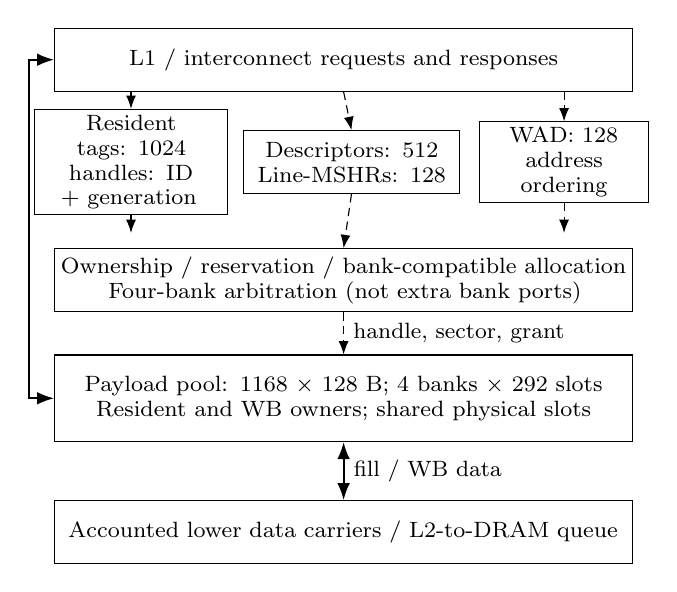
\begin{tikzpicture}[x=1mm,y=1mm,>=Latex,font=\fontsize{8}{9}\selectfont,
box/.style={draw,align=center,inner sep=2pt,minimum height=8mm},
ctl/.style={->,densely dashed,line width=.4pt},data/.style={<->,line width=.7pt}]
\node[box,text width=72mm] (in) at (40,53) {L1 / interconnect requests and responses};
\node[box,text width=23mm] (tag) at (13,40) {Resident tags: 1024\\handles: ID + generation};
\node[box,text width=26mm] (req) at (41,40) {Descriptors: 512\\Line-MSHRs: 128};
\node[box,text width=20mm] (wad) at (68,40) {WAD: 128\\address ordering};
\node[box,text width=72mm] (ctrl) at (40,25) {Ownership / reservation / bank-compatible allocation\\Four-bank arbitration (not extra bank ports)};
\node[box,text width=72mm,minimum height=11mm] (pool) at (40,10) {Payload pool: 1168 $\times$ 128 B; 4 banks $\times$ 292 slots\\Resident and WB owners; shared physical slots};
\node[box,text width=72mm] (low) at (40,-7) {Accounted lower data carriers / L2-to-DRAM queue};
\draw[ctl] (in.south)--(req.north);
\draw[ctl] (13,49)--(tag.north);\draw[ctl] (68,49)--(wad.north);
\draw[ctl] (tag.south)--(13,31);\draw[ctl] (req.south)--(ctrl.north);\draw[ctl] (wad.south)--(68,31);
\draw[ctl] (ctrl.south)--node[right]{handle, sector, grant} (pool.north);
\draw[data] (pool.south)--node[right]{fill / WB data} (low.north);
\draw[data] (in.west)--(0,53)--(0,10)--(pool.west);

\end{tikzpicture}
\end{minipage}\hfill
\begin{minipage}[t]{.49\textwidth}
\centering\small\textbf{(b) Copy removal and separate release events}\par\smallskip
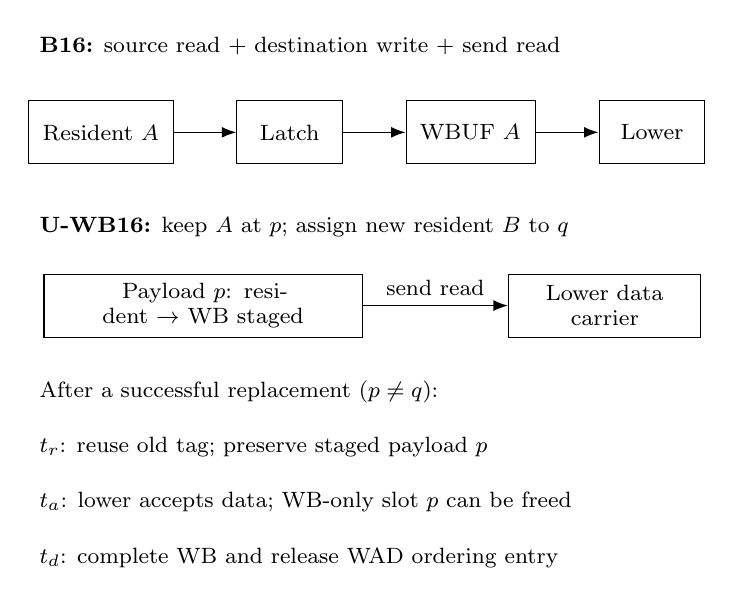
\begin{tikzpicture}[x=1mm,y=1mm,>=Latex,font=\fontsize{8}{9}\selectfont,
box/.style={draw,align=center,inner sep=2pt,minimum height=8mm},arr/.style={->,line width=.5pt}]
\node[anchor=west] at (0,55) {\textbf{B16:} source read $+$ destination write $+$ send read};
\node[box,text width=17mm] (a) at (9,44) {Resident $A$};
\node[box,text width=12mm] (l) at (33,44) {Latch};
\node[box,text width=15mm] (w) at (56,44) {WBUF $A$};
\node[box,text width=12mm] (d) at (79,44) {Lower};
\draw[arr] (a)--(l);\draw[arr] (l)--(w);\draw[arr] (w)--(d);
\node[anchor=west] at (0,32) {\textbf{U-WB16:} keep $A$ at $p$; assign new resident $B$ to $q$};
\node[box,text width=39mm] (p) at (22,22) {Payload $p$: resident $\to$ WB staged};
\node[box,text width=23mm] (lo) at (73,22) {Lower data carrier};
\draw[arr] (p)--node[above]{send read} (lo);
\node[anchor=west] at (0,11) {After a successful replacement ($p\ne q$):};
\node[anchor=west] at (0,4) {$t_r$: reuse old tag; preserve staged payload $p$};
\node[anchor=west] at (0,-3) {$t_a$: lower accepts data; WB-only slot $p$ can be freed};
\node[anchor=west] at (0,-10) {$t_d$: complete WB and release WAD ordering entry};
\end{tikzpicture}
\end{minipage}
\caption{From relocation to ownership transfer. (a) Resident tags, requester descriptors, and writeback address ordering are separately tracked around a fixed banked payload pool. (b) B16 copies an evicted dirty line to its WBUF; U-WB retains the bytes at $p$ while allocating a different landing $q$ for the incoming resident. Local storage is released after lower data acceptance, whereas address ordering persists to writeback completion. Both modes have equal data capacity, bank service, and a common copy latch. TVD/RO and concurrent dynamic bypass are outside the reported WB-only evaluation.}
\label{fig:organization}
\end{figure*}


Figure~\ref{fig:organization} shows the declared service model. WB-only pooling can borrow reference bypass-return slots, but concurrent dynamic bypass use is unvalidated. Idle bypass capacity therefore makes a WB-heavy static control important.

A resident tag names a payload through a slot identifier and generation. Each slot has one authoritative owner; ready/pending sector masks and pins track its consumers. The initial design preserves the resident bank class:
\begin{equation}
 \operatorname{bank}(p)=p\bmod4=\operatorname{tag\_index}\bmod4.
\label{eq:bank}
\end{equation}
A globally free slot is therefore not necessarily a legal landing for a given tag. The 1024 tags bound resident visibility; a temporarily reserved incoming landing is not an additional visible resident line.

\subsection{Eviction as an Ownership Transfer}
For a dirty victim $A$ held in payload $p$, B16 performs a resident read and WBUF write before the eventual send read. U-WB16 instead converts the owner of $p$ from resident to \texttt{WB\_STAGED}, leaving the bytes in place, and reserves a distinct slot $q\ne p$ for the incoming resident $B$. Because each tag has a fixed bank class, a free landing must belong to that same bank. A successful transfer saves the two copy operations, but does not eliminate the send read or the lower-level data carrier.

This transition is performed as one serialized replacement transaction. Before reserving any state, the frontend checks required miss-queue capacity, outstanding pins and sectors, WAD availability, and legal staging and landing slots. For a pending replacement it records the requester, chosen tag index, old payload handle, and acquired resources. A later tag probe by the \emph{same request} uses the held victim index, even when a fill in another way has changed the raw LRU candidate. Preview and native tag access therefore agree across bank retries. Other frontend requests cannot take over that pending transaction.

The tag-to-payload remapping is committed only after the necessary bank work is granted. If native access subsequently refuses the replacement, the controller rolls back uncommitted reservations and restores the old payload/tag identity; bank work already performed is still accounted for. Source-bound tests exercise competing fills, cross-cycle victim identity, and the unchanged one-operation-per-bank service rule.

\subsection{Progress and Independent Retirement}
The ownership transfer does not make writeback instantaneous (Fig.~\ref{fig:organization}). At replacement commit $t_r$, the old tag can be reused while payload $p$ remains \texttt{WB\_STAGED}. At actual downstream acceptance $t_a$, the lower queue assumes responsibility for carrying the dirty bytes and the local slot can be released. The WAD record survives until writeback completion $t_d$ to preserve same-address ordering. Local payload storage and ordering metadata are thus reclaimed according to different last consumers.

Outstanding reads follow the same ownership discipline: requester descriptors and payload pins remain live until their responses are accepted. Generation identity, per-sector readiness, and complete resource drain are validated separately.

\begin{figure*}[t]
\centering
\includegraphics[width=\textwidth]{figures/fig2_results.pdf}
\caption{Five independently received H0 native pairs, unchanged by diagnostic conditions. (a) Cycle reduction $100(C_B-C_U)/C_B$, on an expanded scale with zero denoting B16; CFD regression is retained. The speed-ratio geomean is 1.001600, not the mean of these percentages. (b) Actual completed 128-B copies; U-WB16 is zero in every pair. Vector, Conv., and FWT denote vectorAdd\_4M, convolutionSeparable, and FWT\_7\_21. No error bars or significance claim.}
\label{fig:mainresults}
\end{figure*}

\subsection{Implementation Cost and Extension Boundary}
The pool stores 146 KiB per L2 slice, or 9.125 MiB over 64 slices; each slice also has the same explicitly modeled 128-B copy latch in both designs. An 11-bit slot index names one of 1168 payload locations; generation and owner state accompany tag and WB handles. Some fields already exist in the reference, so the gross handle bit counts cannot be interpreted as incremental silicon area. The real added cost includes handle selection, bank-compatible allocation, ownership checks, pins, and transaction control. Equal modeled data capacity and bank throughput do not establish equal hit latency, circuit timing, area, or energy. No RTL synthesis, STA, or measured power is claimed.

Transient-victim retention (TVD) and certified read-only bypass (RO) are separate potential clients of a decoupled payload design, but neither is enabled or scientifically qualified in the present WB-only application results.

\section{Experimental Methodology}
\subsection{Matched Resources and Complete Inputs}
We use the Accel-Sim SASS flow and GPGPU-Sim performance-model lineage~\cite{accelsim,gpgpusim}. Their published validation does not validate this modified L2. B16 and U-WB16 must execute with the same independently qualified binary, complete trace input, non-mode settings, timing scope, and termination rules. Table~\ref{tab:configuration} records the current ordered research configuration, including the modified L2; it is not a reconstruction of undocumented commercial-cache internals.

\begin{table}[t]
\caption{Declared matched configuration. L2 capacities are per slice.}
\label{tab:configuration}\centering\footnotesize
\begin{tabularx}{\columnwidth}{@{}L{.42\columnwidth}X@{}}
\toprule
Resource & Setting \\
\midrule
Compute / clock domains & 80 SMs; core/ICNT/L2: 1132 MHz; DRAM: 850 MHz \\
L1 (fixed) & 64 KiB/SM; 4 banks; 20-cycle setting \\
L2 tags / data & 1024 tags; 1168 slots, 146 KiB \\
Line / sectors / banks & 128 B / $4\times32$ B / $4\times292$ slots \\
Service / common latch & 1 op/bank/physical cycle / 128 B \\
Descriptors / Line-MSHRs & 512 / 128; 32 requesters/address \\
WAD / lower queue & 128 / 128 entries \\
Chip / memory channels & 64 slices / 32 channels \\
L2 ROP delay & 160-cycle model setting \\
DRAM scheduler / return & 128 / 192 entries per channel \\
\bottomrule
\end{tabularx}
\end{table}

The fixed development set is convolutionSeparable, FWT\_7\_21, cfd\_097k, vectorAdd\_4M, and SAD. Accepted manifests bind each complete commandlist, input size, and trace body; workload names alone are insufficient. SAD is the predeclared negative control. All five pairs, including slowdowns, enter the geometric mean. This development set does not establish holdout or general GPU coverage.

\subsection{Validation Boundary}
B16 and U-WB16 run the same simulator executable, complete original commandlists and trace bodies, and identical non-mode settings. Production and independent tests exercise cross-cycle replacement, physical-cycle bank grants, symbolic 32-B sector versions, host prefill, response backpressure, and distinct writeback acceptance and completion. Every qualified run closes its outstanding requests and resource trackers. Complete native opcode auditing restricts these experiments to non-atomic inputs. Since SASS traces lack full numerical payload values, these tests establish transaction and lifecycle consistency rather than numerical application-output correctness. The complete input, binary, configuration, log, and check identities are preserved in the reproducibility artifacts.

\section{From Saved Internal Work to Application Effects}
\subsection{Copy Removal Is Not a Speedup Model}
All five predeclared H0 workload pairs have complete trace-driven simulation results and pass the stated transaction-lifecycle checks. Each pair has equal instruction counts and matched full input/termination scope. Figure~\ref{fig:mainresults}(a) reports the complete set: SAD is almost tied; Vector, Convolution, and FWT reduce cycles by 0.199\%, 0.480\%, and 0.310\%, while CFD increases cycles by 0.214\%. The geometric mean of $C_B/C_U$ is 1.001600, or a 0.160\% speed-ratio gain. These deterministic paired observations establish neither statistical significance nor general GPU speedup. Exact paired cycles and reproducibility identities accompany the evaluation artifacts.

Figure~\ref{fig:mainresults}(b) shows removal of every measured resident-to-WB copy. A committed non-rolled-back B16 writeback uses two copy operations and one send read; U-WB16 retains the send read. This local operation saving is not a speedup model. Actual WB counts also change: CFD completes 31,123/31,063 WBs and FWT 178,569/178,585 for B16/U-WB16. Consequently, the run-level logical-operation difference need not equal twice either mode's WB count. Artifact tables preserve actual WB/send-read and DRAM-byte totals.

\begin{figure*}[t]
\centering
\includegraphics[width=\textwidth]{figures/fig3_pressure.pdf}
\caption{H0 application-cumulative pressure and service observations. (a) WB-data-full refusal attempts; CFD's small B16 count is labeled explicitly. (b) Separate relative reductions in logical work/successful modeled bank grants and in summed per-operation conflict waits. Logical operations and grants coincide at drain in these runs, but are independently checked counters. (c) Frontend attempts denied when the L2-to-DRAM queue is full. M denotes $10^6$. Attempt counts and operation-wait sums are not elapsed GPU cycles or unique transactions; reductions and increases do not establish causality.}
\label{fig:causal}
\end{figure*}

\subsection{Local Staging Relief and Its Downstream Cost}
Vector, Convolution, and FWT record 440,161, 845,097, and 890,294 B16 WB-data-full events; U-WB16 records zero. Figure~\ref{fig:causal}(b) shows less modeled bank work and lower aggregate conflict waits. Successful grants are actual model-service observations, not estimates obtained by multiplying copies. At drained termination, their equality to logical operations implies neither elapsed-time nor RTL timing/energy savings.

For the same three workloads, L2-to-DRAM full-block attempts rise from 1.104M to 1.764M, 0.218M to 1.132M, and 0.013M to 0.968M. This is consistent with pressure moving downstream after local staging relief. It does not independently identify the limiting queue or DRAM service. Denials may repeat for one frontend head and overlap other blockers. From final cumulative observations of all 32 channels, the modeled issued-byte/atom-cycle fractions are 64.5/64.8\% for Convolution and 14.1/14.1\% for FWT. Even frequent queue denials therefore do not prove global DRAM-bandwidth saturation. Kernel-boundary cumulative snapshots are not summed.

CFD is a useful counterexample: despite removing copies and lowering bank waits from 102,546 to 91,029, U-WB16 takes 169 more cycles. WAD-hazard events increase from 9,841 to 13,400, WB counts differ, and successful DRAM writes change from 3,983,744 to 3,976,064~B. These correlated changes motivate ordering/service diagnosis; they do not identify a unique cause. SAD has no observed WB-data-full pressure and differs by only 24 cycles. Neither case is discarded.



\subsection{Separating Buffer Headroom from Service Speed}
The local WBUF limit may cease to matter once the backend becomes faster, or the backend may prevent either mode from realizing its freed bank work. To distinguish these possibilities, we define two matched downstream conditions for Convolution and FWT. Q4 increases lower queue/scheduler/return buffering and its derived credits; D4 keeps Q4 and raises the modeled DRAM clock domain. Both interventions apply equally to B16 and U-WB16, without changing the L2 data pool or bank service. The extra storage and altered DRAM timing are not free hardware or a pure bandwidth change~\cite{sms}.

For workload $w$ and condition $h$, the within-condition mechanism effect is $S_w(h)=C_{B,w}(h)/C_{U,w}(h)$; the interaction with H0 is $J_w(h)=S_w(h)/S_w(\mathrm{H0})$. Speeding up both designs does not by itself enlarge U-WB's advantage, and a faster backend can also reduce the reference's WBUF residence. These tests characterize an operating regime, not a production DRAM-frequency recommendation.

\begin{table}[t]
\caption{Matched downstream sensitivity settings for Convolution and FWT; experiment results are distinct from the H0 five-workload cohort.}
\label{tab:headroom}\centering\footnotesize
\begin{tabular}{@{}lrrr@{}}
\toprule
Resource & H0 & Q4 & D4 \\
\midrule
L2$\to$DRAM / DRAM$\to$L2 & 128/64 & 512/256 & 512/256 \\
Scheduler / return queues & 128/192 & 512/768 & 512/768 \\
Derived shared credits & 319 & 1279 & 1279 \\
DRAM clock (MHz) & 850 & 850 & 3400 \\
\bottomrule
\end{tabular}
\end{table}

The original H0 cohort is retained regardless of later sensitivity results. A separate equal-capacity static repartition is still needed to show that dynamic pooling is preferable to a better fixed WB quota.

\section{Relation to Prior Storage Decoupling}
The Virtual Write Queue exposes LLC dirty-line candidates to DRAM scheduling while retaining a physical write queue~\cite{vwq}. Decoupled last-write prediction keeps candidate addresses in a last-write buffer and data in the LLC; evicted dirty blocks use a separate write buffer~\cite{lastwrite}. The Dirty-Block Index (DBI) separates dirty bits from tags and groups them by DRAM row~\cite{dbi}. Their contributions concern candidate visibility, early cleaning, or dirty-state indexing; EP-L2 instead concerns the original payload slot's owner after the resident tag is reused, together with a distinct incoming landing and separate payload/order retirement. DBI dirty status is not the WAD's in-flight same-address ordering state.

V-Way decouples tag/data placement~\cite{vway}; Tag-Split Cache separates request and storage granularity~\cite{tsc}. Gebhart et al. unify SM-local register, cache, and scratchpad storage~\cite{unified}. In-cache MSHRs~\cite{farkas}, MiCache's shared FPGA data/MSHR storage~\cite{micache}, and DL-MSHR's linked slots, including write-miss data~\cite{dlmshr}, motivate distinguishing what is shared. Our comparison fixes resident-tag and miss-tracking budgets; it evaluates dirty-payload ownership rather than extra lookup or request-tracking capacity.

\section{Conclusion}
Eviction need not force dirty data to move simply because a tag becomes reusable. EP-L2 turns that event into an ownership transfer: an evicted dirty line retains its slot, a new resident receives a legal landing, and local data storage and address-ordering state retire when their respective consumers finish. The protocol removes relocation work at a fixed payload capacity and modeled bank-service budget. Across five complete trace-driven workloads, every observed resident-to-WBUF copy disappears and three workloads avoid the reference WBUF-data limit, yet the geometric-mean speed ratio is only 1.0016. The central result is a distinction between \emph{internal storage efficiency} and \emph{system-level performance}: the latter depends on whether copy work and staging quotas lie on the critical path, and on the surrounding memory service. Determining the competitive static allocation and the physical cost of this flexibility remains essential before claiming a general advantage.

% Keep the optional fifth page reference-only. No technical appendix on that page.
\clearpage
\bibliographystyle{IEEEtran}
\bibliography{references_verified}
\end{document}
